\documentclass{article}
\usepackage{graphicx} % Required for inserting images
\usepackage{graphicx}
\usepackage{subcaption}
\usepackage{float}
\usepackage[a4paper,margin=1.5cm]{geometry}
\usepackage{tabularx}
\usepackage{pgfplots}
\pgfplotsset{compat=1.18}
\usepgfplotslibrary{statistics}
\usepackage{tikz}
\usepackage{float}





\usepackage{graphicx}
\setkeys{Gin}{height=5cm,keepaspectratio}


\title{Benchmarking Calorie and Nutrient Tracking Apps}
\author{Joana Silva}
\date{January 2026}

\begin{document}

\maketitle

\section{Introduction}
The following report presents a comparative evaluation of existing calorie and nutrient tracking applications, with the objective of doing a market study of the NutriAI competitors available, studying what does NutriAi do better and opportunities for improvement relevant to the development of a new application in this domain.

For this study, the following applications were selected for evaluation: MyFitnessPal,  Calorie \& Protein Tracker Arise, Calorix AI, and Calorie Cue. These applications were chosen due to their functional similarity to NutriAI and their integration of AI-based features, which aligns with the objectives of the course \emph{Foundations and Applications of Generative AI}. The analysis aims to assess how such features are currently implemented and seeing from a user perspective how they work. 

A fixed evaluation framework was applied uniformly across all applications, covering the following aspects: Food Database and Accuracy; Nutrient Coverage; Logging and Input Methods; Goal Setting and Feedback; Usability and User Experience; Data Export and Integrations; and Limitations and Constraints. For each application, the on-boarding process was completed, a user profile was created, and identical tasks were performed, including logging the same meals, packaged foods, and custom recipes, as well as reviewing daily and weekly summaries. All tests were conducted on an Apple iPhone~15 running iOS~26.0, using the most recent free version of each application. The resulting analysis is presented by application, followed by a comparative synthesis and a positioning of NutriAI relative to the evaluated solutions.

\section{Food Database and Accuracy}
\subsection{Ground-Truth Accuracy Evaluation}

To impartially evaluate the accuracy of the applications, a set of meals from an external dataset containing a photograph, a short textual description, and ground-truth nutritional values was used across all apps. To avoid overextending this report, only the results for \emph{Meal~01} are presented.

Description: A chicken thigh with wild rice, red onion, carrots, herbs, and a small amount of lemon.

Photo:
\begin{figure}[H]
    \centering
    \includegraphics[width=0.5\linewidth]{meal_01.jpg}
    \caption{Test Meal 01}
    \label{fig:meal01}
\end{figure}


Nutritional values: 
\begin{table}[H]
\centering
\begin{tabular}{l c}
\hline
\textbf{Metric} & \textbf{Value} \\
\hline
Total calories (kcal) & 377 \\
Carbohydrates (g) & 42 \\
Protein (g) & 24 \\
Fat (g) & 13 \\
\hline
\end{tabular}
\caption{Ground-truth nutritional values for Test Meal~01}
\label{tab:ground_truth_meal}
\end{table}


\subsection{MyFitnesssPal}
The database contains approximately 14 million food entries, including both verified and user-generated items. Verified entries are clearly identified with a visual marker, and for common foods, a substantial number of verified options are available in the free version. For branded products or complete meals, user-generated entries were more frequently required, as multiple entries representing the same item exhibited variations in nutritional values.

Multiple duplicated entries were observed for identical food items, particularly among user-generated entries, often with ambiguous naming conventions. This requires manual selection by the user and increases the likelihood of inaccurate logging due to discrepancies between entries representing the same item. In contrast, duplicated verified entries were observed less frequently, and when present, the associated nutritional values showed only minor variation.

Small nutritional discrepancies were observed between different verified entries representing the same food item, with caloric values differing by approximately 8\%, indicating limited variability in data accuracy. For most food items, the data source is not explicitly stated, although entries are often organized by brand, allowing users to search for specific products.

\begin{figure}[H]
    \centering
    \begin{subfigure}[t]{0.22\textwidth}
        \centering
        \includegraphics[width=\linewidth]{WhatsApp Image 2026-01-20 at 12.50.52.jpeg}
        \caption{Banana — Verified entry 1}
        \label{fig:MFP_banana_verified_1}
    \end{subfigure}
    \hspace{0.02\textwidth}
    \begin{subfigure}[t]{0.22\textwidth}
        \centering
        \includegraphics[width=\linewidth]{WhatsApp Image 2026-01-20 at 12.50.53.jpeg}
        \caption{Banana — Verified entry 2}
        \label{fig:MFP_banana_verified_2}
    \end{subfigure}
    \caption{Verified entries for ``banana'' in the MyFitnessPal application}
    \label{fig:MFP_banana_verified_comparison}
\end{figure}

For a verified branded food item (KitKat bar)it was a perfect match between value reported in the application (212 kcal) and the value indicated on the product label (212 kcal).

\begin{figure}[H]
    \centering
    \begin{subfigure}[t]{0.22\textwidth}
        \centering
        \includegraphics[width=\linewidth]{WhatsApp Image 2026-01-20 at 16.43.39.jpeg}
        \caption{KitKat- verified entry}
        \label{fig:mfp_KitKat_verified}
    \end{subfigure}
    \hspace{0.02\textwidth}
    \begin{subfigure}[t]{0.22\textwidth}
        \centering
        \includegraphics[width=\linewidth]{034000002467_7.jpg}
        \caption{Kitkat-Label}
        \label{fig:KitKat_label}
    \end{subfigure}
    \caption{MyFitnessPal App Info vs. Brand Label}
    \label{fig:MFP_KitKat_comparison}
\end{figure}

To evaluate nutritional accuracy under controlled conditions, a ground-truth dataset was used as reference, containing the true caloric and macronutrient values for a composed meal. The meal consisted of a chicken thigh with wild rice, red onion, carrots, herbs, and a small amount of lemon. All food items were manually logged in the application using verified entries only, without prior knowledge of the exact quantities or nutritional values, and without relying on any automatic food recognition or estimation features.

For this meal, the ground-truth values were 377 kcal, 42 g of carbohydrates, 24 g of protein, and 13 g of fat. Using MyFitnessPal, the manually logged meal resulted in a total of 421 kcal, with 46.2 g of carbohydrates, 26.7 g of protein, and 13 g of fat. While the fat content matched the reference value, the application overestimated total calories and carbohydrates, indicating a moderate deviation when ingredient quantities are inferred manually. This result highlights the sensitivity of nutritional accuracy to portion size assumptions, even when verified database entries are used.

\begin{figure}[H]
    \centering
    \begin{subfigure}[t]{0.3\textwidth}
        \centering
        \includegraphics[width=\linewidth]{
        WhatsApp Image 2026-01-20 at 20.28.49(2).jpeg}
        \caption{Meal 01- input}
        \label{fig:MFP_meal01-calories}
    \end{subfigure}
    \hfill
    \begin{subfigure}[t]{0.3\textwidth}
        \centering
        \includegraphics[width=\linewidth]{WhatsApp Image 2026-01-20 at 20.28.49(1).jpeg}
        \caption{Meal01- ingredients entries}
        \label{fig:MFP_meal01-ingredients1}
    \end{subfigure}
    \hfill
    \begin{subfigure}[t]{0.3\textwidth}
        \centering
        \includegraphics[width=\linewidth]{WhatsApp Image 2026-01-20 at 20.28.49.jpeg}
        \caption{Meal01- ingredients entries}
        \label{fig:MFP_meal01-ingredients2}
    \end{subfigure}
    \caption{FitnessPal App- Accuracy Test}
    \label{fig:MFP_daily_summary_comparison}
\end{figure}



\subsection{arise}
The arise application relies exclusively on user-generated food entries, with no verified items available in its food database. No visual distinction is provided between different entry types, and the overall database size is not stated. The payed version had a color code for different entries with their energy density:  having 3 categories:"you may eat plenty", "eat moderate amounts" or "stay with small amounts".  During testing, multiple duplicate entries were observed for identical food items, contributing to ambiguity during manual food selection. Significant nutritional discrepancies were identified when comparing different entries for the same food. For example, two entries for a simple food item exhibited caloric values of 98 kcal and 40 kcal, indicating substantial inconsistency. Also, The app allows different database languages, by default my app was in portuguese (even though everything on the app was in english), when changing the database to english it was possible to see more different entries for the same item with different nutritional values: the same item that was 98 kcal to 40 kcal in the portuguese database in the english database it went from 82 kcal to 176 kcal.


\begin{figure}[H]
    \centering
    \begin{subfigure}[t]{0.22\textwidth}
        \centering
        \includegraphics[width=\linewidth]{WhatsApp Image 2026-01-20 at 21.50.43.jpeg}
        \caption{Banana — different entries- portuguese database}
        \label{fig:arise_banana}
    \end{subfigure}
     \hspace{0.02\textwidth}
    \begin{subfigure}[t]{0.22\textwidth}
        \centering
        \includegraphics[width=\linewidth]{WhatsApp Image 2026-01-20 at 12.50.53.jpeg}
        \caption{Banana — different entries- english database}
        \label{fig:arise_banana_2}
    \end{subfigure}
    \caption{Entries for ``banana'' in the arise application}
    \label{fig:arise_banana_comparison}
\end{figure}


For branded products such as KitKat, discrepancies were also observed. A user-created entry reported 223 kcal, compared to 212 kcal stated on the product label, while barcode-based logging resulted in a value of 183 kcal. These results indicate considerable variability depending on the logging method and selected entry.

\begin{figure}[H]
    \centering
    \begin{subfigure}[t]{0.3\textwidth}
        \centering
        \includegraphics[width=\linewidth]{WhatsApp Image 2026-01-20 at 21.58.59.jpeg}
        \caption{KitKat-user input}
        \label{fig:MFP_meal01-calories}
    \end{subfigure}
    \hfill
    \begin{subfigure}[t]{0.3\textwidth}
        \centering
        \includegraphics[width=\linewidth]{WhatsApp Image 2026-01-20 at 21.59.27.jpeg}
        \caption{KitKat- barcode read}
        \label{fig:MFP_meal01-ingredients1}
    \end{subfigure}
    \hfill
    \begin{subfigure}[t]{0.3\textwidth}
        \centering
        \includegraphics[width=\linewidth]{034000002467_7.jpg}
        \caption{Kitkat-Label}
        \label{fig:KitKat-label}
    \end{subfigure}
    \caption{arise App Info vs. Brand Label}
    \label{fig:ARISE_KitKat_comparison}
\end{figure}


No explicit information regarding data sources or brand-based organization was provided. Overall, the absence of verified entries and data transparency increases the likelihood of inaccurate nutritional logging.

To assess nutritional accuracy under controlled conditions, a ground-truth dataset containing known caloric and macronutrient values for a composed meal was used as reference.

To test the nutritional accuracy under controlled conditions, a ground-truth dataset was used as reference, containing the true caloric and macronutrient values for a composed meal. It was used the scan meal tool built in the free version of the app.
The app allows different database languages, by default my app was in portuguese (even though everything on the app was in english). When first scanning the meal (with portuguese database) the results were as following: 
\begin{figure}[H]
    \centering
        \centering
        \includegraphics[width=\linewidth]{resultado-pt.jpeg}
        \caption{Meal 01- Photo scan- Portuguese Database}
        \label{arise_pt_meal01-calories}
\end{figure}

The ingridients listed were: 150g Roasted chicken thigh (339kcal), 120g Wild rice (150kcal), boiled 60g carrot(21 kcal), 30g Celary (5kcal), 40g Lemon (12kcal), 10ml olive oil (90kcal)
After the first photo scan it was introduced the description of the meal in the "fix" AI bottom the AI made the following changes: 
\begin{figure}[H]
    \centering
    \begin{subfigure}[t]{0.22\textwidth}
        \centering
        \includegraphics[width=\linewidth]{fix.jpeg}
        \caption{Description}
        \label{fig:arise_fix}
    \end{subfigure}
    \hspace{0.02\textwidth}
    \begin{subfigure}[t]{0.22\textwidth}
        \centering
        \includegraphics[width=\linewidth]{correcao-pt.jpeg}
        \caption{Meal 01- After prompt- Portuguese DataBase}
        \label{fig:arise_pt_meal01_fix}
    \end{subfigure}
    \caption{Meal 01- AI fix- Portuguese Database}
    \label{fig:arise_fix_pt}
\end{figure}

The ingredients listed this time were: 20g Red onion (8kcal), 30g Celary(4,8kcal), 30g Lemon (8,7kcal), 10ml olive oil (90kcal), 2g fresh herbs (2,6kcal)


For my surprise when the database was changed to english and the same procedure was implemented the results were different: 
\begin{figure}[H]
    \centering
        \centering
        \includegraphics[width=\linewidth]{resultado-ingles.jpeg}
        \caption{Meal 01- Photo scan- English Database}
        \label{arise_eng_meal01-calories}
\end{figure}




The ingridients listed for the english version were: 150g Roasted chicken thigh (315,5 kcal), 120g Wild rice mix (156 kcal), 60g Carrots (24,6 kcal), 20g red onion (8kcal), 30g celery (4,8 kcal), 30g lemon (8,7kcal), 10ml olive oil (90 kcal) and 2g fresh herbs (2,6 kcal). 
Then the same prompt was implemented in the fix feature. the results were as follows:
\begin{figure}[H]
    \centering
        \centering
        \includegraphics[width=\linewidth]{correcao-ingles.jpeg}
        \caption{Meal 01- After prompt- English DataBase}
        \label{fig:arise_eng_meal01_fix}
    \label{fig:arise_fix_eng}
\end{figure}

The ingridients listed for the prompted english version were: 150g Roasted chicken thigh (315,5 kcal), 120g Wild rice mix (156 kcal), 60g Carrots (24,6 kcal), 30g celery (4,8 kcal),10ml olive oil (88,2kcal) and 40g Lemon (11,6 kcal). 

Results indicate that photo-based meal recognition is highly sensitive to database language selection and AI prompt refinement, leading to caloric overestimations of more than 50\% relative to the ground-truth value for the same meal. While MyFitnessPal overestimated the ground-truth caloric value by approximately 12\% using manual logging, photo-based scanning methods produced overestimations exceeding 50\%, with results highly dependent on database language and AI refinement.
\subsection{Calorix AI}

The application provides a food database with over two million entries, composed of a single, unspecified entry type, which appears to be user-generated, as users are able to create new food items. No verified entries or explicit data source information are provided. During testing, duplicate entries were observed for identical food items, contributing to ambiguity during manual selection.

Moderate discrepancies were identified for simple food items, such as bananas, with caloric values of 105 kcal and 110 kcal across different entries. 


\begin{figure}[H]
        \centering
        \includegraphics[width=\linewidth]{banana_calorix.jpeg}
        \caption{Entries for ``banana'' in the Calorix AI application}
        \label{fig:calorix_banana}
\end{figure}

For branded products, variability depended on the logging method. A manually selected entry for a KitKat bar reported 178 kcal, compared to 212 kcal on the product label, whereas barcode-based logging produced a value of 213 kcal, closely matching the reference value. These results indicate that barcode scanning improves accuracy relative to manual entry in the absence of verified items.

\begin{figure}[H]
    \centering
    \begin{subfigure}[t]{0.3\textwidth}
        \centering
        \includegraphics[width=\linewidth]{kitkat_calorixentry.jpeg}
        \caption{KitKat-user input}
        \label{fig:MFP_meal01-calories}
    \end{subfigure}
    \hfill
    \begin{subfigure}[t]{0.3\textwidth}
        \centering
        \includegraphics[width=\linewidth]{kitkat_calorixbarcode.jpeg}
        \caption{KitKat- barcode read}
        \label{fig:MFP_meal01-ingredients1}
    \end{subfigure}
    \hfill
    \begin{subfigure}[t]{0.3\textwidth}
        \centering
        \includegraphics[width=\linewidth]{034000002467_7.jpg}
        \caption{Kitkat-Label}
        \label{fig:KitKat-label}
    \end{subfigure}
    \caption{Calorix AI App Info vs. Brand Label}
    \label{fig:ARISE_KitKat_comparison}
\end{figure}

To evaluate nutritional accuracy under controlled conditions,as in the other apps Meal01 was used. The meal was logged using a textual description, as voice-based input repeatedly caused application crashes and image-based meal scanning was restricted to the paid version. Quantities were not known beforehand, and values were generated automatically based on the provided description.

 \begin{figure}[H]
    \centering
        \centering
        \includegraphics[width=\linewidth]{meal01-calorix-prompt.jpeg}
        \caption{Meal 01- Text Description}
        \label{calorix-meal-01-prompt}
\end{figure}

The application reported a total of 370 kcal, compared to the ground-truth value of 377 kcal, resulting in a deviation of approximately 2\%. Protein values were similarly close to the reference, while fat content was moderately overestimated. In contrast, carbohydrate content exhibited a substantial deviation, representing the largest source of error. These results suggest that AI-based text interpretation can yield accurate caloric estimates overall, but remains sensitive to portion size assumptions, particularly for carbohydrate-rich ingredients.

\begin{figure}[H]
    \centering
    \begin{subfigure}[t]{0.22\textwidth}
        \centering
        \includegraphics[width=\linewidth]{calorix-meal01-ingredients.jpeg}
        \caption{Ingridents detected}
        \label{fig:arise_fix}
    \end{subfigure}
    \hspace{0.02\textwidth}
    \begin{subfigure}[t]{0.22\textwidth}
        \centering
        \includegraphics[width=\linewidth]{calorix-meal01-results.jpeg}
        \caption{Meal 01 Overall Analysis}
        \label{fig:arise_pt_meal01_fix}
    \end{subfigure}
    \caption{Calorix AI App- Accuracy Test}
    \label{fig:arise_fix_pt}
\end{figure}

\subsection{Calorie Cue}

The Calorie Cue application provides a food database composed exclusively of verified entries, with no support for user-generated food items.Even though the user can generate their own food entries and acess to those unverified ones. Entry types are visually distinguishable, and no duplicate food items were observed during testing. Although the total database size is not explicitly stated, the organization includes branded products and restaurants, supporting brand-based searches.

For branded food items, consistency depended on the logging method. Barcode-based logging for a KitKat bar reported 213 kcal, closely matching the label value of 212 kcal. However, manual database search returned an entry reporting 512 kcal for the same product, indicating a substantial discrepancy.

\begin{figure}[H]
    \centering
    \begin{subfigure}[t]{0.3\textwidth}
        \centering
        \includegraphics[width=\linewidth]{kitkat-appsearch-cue.jpeg}
        \caption{KitKat-app verified entrance}
        \label{fig:cuekitkat1}
    \end{subfigure}
    \hfill
    \begin{subfigure}[t]{0.3\textwidth}
        \centering
        \includegraphics[width=\linewidth]{kitkat-barscan-cue.jpeg}
        \caption{KitKat- barcode read}
        \label{fig:cuekitkat2}
    \end{subfigure}
    \hfill
    \begin{subfigure}[t]{0.3\textwidth}
        \centering
        \includegraphics[width=\linewidth]{034000002467_7.jpg}
        \caption{Kitkat-Label}
        \label{fig:KitKat-label}
    \end{subfigure}
    \caption{cue App Info vs. Brand Label}
    \label{fig:cue_KitKat_comparison}
\end{figure}

Nutritional accuracy was evaluated using the same composed meal from the external ground-truth dataset. Meal logging relied exclusively on photo-based scanning, as this was the primary supported input method. Ingredient quantities were not known beforehand, and nutritional values were automatically inferred by the application.

The application reported a total caloric value of 453 kcal, exceeding the ground-truth value of 377 kcal by 73 kcal (approximately 19\%). The largest deviation was observed for carbohydrates, while protein and fat values remained close to the reference. These discrepancies are likely attributable to portion size assumptions made during AI-based image interpretation.

\begin{figure}[H]
    \centering
    \begin{subfigure}[t]{0.22\textwidth}
        \centering
        \includegraphics[width=\linewidth]{scanmeal-cue1.jpeg}
        \label{fig:cue_fix}
    \end{subfigure}
    \hspace{0.02\textwidth}
    \begin{subfigure}[t]{0.22\textwidth}
        \centering
        \includegraphics[width=\linewidth]{scanmeal-cue2.jpeg}
        \label{fig:cue_pt_meal01_fix}
    \end{subfigure}
    \caption{Calorie Cue AI App- Accuracy Test}
    \label{fig:arise_fix_pt}
\end{figure}


The ingredients recognized by the app with photo input only were: 100g chicken thigh (200 kcal), 180g wild rice blend (220 kcal), 60g carrots (25g), 10g lemon (3 kcal). 



\section{Nutrient Coverage}
\subsection{MyFitnessPal}
After logging meals, the application provides a per-meal caloric breakdown on the main interface, distinguishing between breakfast, lunch, dinner, and snacks. In addition, a detailed daily summary of macronutrients and selected nutrients is available, along with a comparison between consumed values and those recommended according to the user’s defined goal.

The application also generates predictive feedback based on the logged caloric intake and physical activity. However, predictions derived from a single day of data may not accurately reflect longer-term dietary patterns, particularly when the logged day corresponds to a typical intake, potentially limiting the reliability of short-term projections.

Nutrient targets are not manually configurable by the user, as recommended intake values are automatically determined based on profile information and selected goals, reducing user control over individualized nutrient planning.

\begin{figure}[H]
    \centering
    \begin{subfigure}[t]{0.3\textwidth}
        \centering
        \includegraphics[width=\linewidth]{App comparison/WhatsApp Image 2026-01-20 at 12.24.27.jpeg}
        \caption{Daily Calories Graph}
        \label{MFP_caloriestrack}
    \end{subfigure}
    \hfill
    \begin{subfigure}[t]{0.3\textwidth}
        \centering
        \includegraphics[width=\linewidth]{App comparison/WhatsApp Image 2026-01-20 at 12.24.27(1).jpeg}
        \caption{Nutrients Daily Info}
        \label{fig:MFP_nutrientstrack}
    \end{subfigure}
    \hfill
    \begin{subfigure}[t]{0.3\textwidth}
        \centering
        \includegraphics[width=\linewidth]{App comparison/WhatsApp Image 2026-01-20 at 12.24.27(2).jpeg}
        \caption{Macro Daily Info}
        \label{fig:MFP_macrotrack}
    \end{subfigure}
    \caption{Daily summary interfaces in MyFitnessPal App}
    \label{fig:MFP_daily_summary_comparison}
\end{figure}


\subsection{arise}

In the free version, nutrient coverage is limited to total caloric intake. Detailed macronutrient and micronutrient information is restricted to the paid version. While per-meal and daily summaries are available, access is limited to the current day and prior to final submission. Weekly summaries are exclusively available in the paid tier.

Nutrient targets are automatically defined based on the user profile and selected goal, with no option for manual customization. As a result, user control over nutrient planning is limited, particularly in the free version.

\subsection{Calorix AI}
The application provides access to caloric and macronutrient information in the free version, while micronutrient data is not available. Per-meal, daily, and weekly summaries are supported. Nutrient targets are initially defined automatically based on the user profile and selected goal; however, manual adjustment of macronutrient targets is allowed, providing greater user control compared to other evaluated applications.

\begin{figure}[H]
    \centering
    \begin{subfigure}[t]{0.3\textwidth}
        \centering
        \includegraphics[width=\linewidth]{calorix-inferface.jpeg}
        \caption{Dashboard Interface}
        \label{calorix_caloriestrack}
    \end{subfigure}
    \begin{subfigure}[t]{0.3\textwidth}
        \centering
        \includegraphics[width=\linewidth]{calorix-interface2.jpeg}
        \caption{Analytics Interface}
        \label{fig:calorix_nutrientstrack}
    \end{subfigure}
    \caption{Daily summary interfaces in Calorix AI App}
    \label{fig:MFP_daily_summary_comparison}
\end{figure}

\subsection{Calorie Cue}

The application provides access to caloric and macronutrient information, while micronutrient data is not displayed. Per-meal, daily, and weekly summaries are supported, including AI-generated weekly summaries and average values. Nutrient targets are defined automatically based on the user profile and can be manually adjusted.

\begin{figure}[H]
    \centering
    \begin{subfigure}[t]{0.24\textwidth}
        \centering
        \includegraphics[width=\linewidth]{dailyinfo-cue.jpeg}
        \caption{Daily Info}
        \label{fig:cue-daily}
    \end{subfigure}
    \hfill
    \begin{subfigure}[t]{0.24\textwidth}
        \centering
        \includegraphics[width=\linewidth]{insights-cue.jpeg}
        \caption{Insights Page 1}
        \label{fig:cue-nutrientstrack}
    \end{subfigure}
    \hfill
    \begin{subfigure}[t]{0.24\textwidth}
        \centering
        \includegraphics[width=\linewidth]{insights-cue2.jpeg}
        \caption{Insights Page 2}
        \label{fig:cue-macrotrack}
    \end{subfigure}
    \hfill
    \begin{subfigure}[t]{0.24\textwidth}
        \centering
        \includegraphics[width=\linewidth]{summarycue.jpeg}
        \caption{AI summary}
        \label{fig:cue-summary}
    \end{subfigure}
    \caption{Daily summary interfaces in Calorie Cue App}
    \label{fig:MFP_daily_summary_comparison}
\end{figure}


\section{Logging and Input Methods}
\subsection{MyFitnessPal}
The application provides four distinct meal logging methods: manual food search, barcode scanning, voice logging, and meal scanning. In the free version, only manual food search is available, whereas the remaining input methods are restricted to the premium tier. The application also allows users to save recipes from online sources, from the app’s internal database, or to create personal recipes, enabling faster logging when reusing previously saved meals through a dedicated “create a meal” function.

Due to the limitation of the free version to manual entry, meal logging becomes more time-consuming and occasionally requires information that users may not readily have available, such as precise portion sizes or specific product details. During testing, logging a single meal required an average of six user interactions, with frequent manual corrections caused by ambiguous or duplicated search results. The reliance on manual entry in the free version significantly impacts logging efficiency when compared to apps offering unrestricted barcode scanning.

\subsection{arise}
The application supports manual food search, barcode scanning, and AI-based meal scanning. While meal scanning is available in both free and paid versions, only the paid version allows scanned meals to be saved. The free version permits viewing of a single scanned meal per day without saving. Recipe creation is not supported, and saved meals are limited in the free tier.

Logging a single meal required an average of six user interactions, with frequent manual corrections due to ambiguous search results. Not all barcodes were recognized, limiting its reliability as a primary logging method.

\subsection{Calorix AI}
Multiple input methods are supported, including manual food search, barcode scanning, voice-based logging, and recipe creation. Image-based meal scanning is restricted to the paid version. Saved meals and templates are available. Logging a meal required an average of five user interactions, with some manual corrections due to ambiguous search results.

While barcode scanning was available in the free tier, its usage was limited to three scans. Voice-based logging was unreliable, as the application consistently crashed during testing. These restrictions negatively impacted logging efficiency in the free version.

\subsection{Calorie Cue}
The application supports multiple input methods, including manual search, barcode scanning, photo-based meal scanning, recipe creation, and saved foods. Voice-based food logging was not available when manually adding a meal. Meal logging was generally efficient in terms of interaction count, requiring an average of two user actions per meal; however, this apparent efficiency was offset by usability and workflow limitations.

After photo-based meal scanning, users are able to edit via AI the automatically recognized ingredients through an AI-assisted correction interface. While removal or modification of detected ingredients was supported, adding missing ingredients required an indirect workflow: users first had to log the recognized meal, navigate to the corresponding meal category (e.g., lunch or dinner), and only then manually add additional items. This process was not intuitive and increased cognitive load.

\begin{figure}
\centering
    \begin{subfigure}[t]{0.22\textwidth}
        \centering
        \includegraphics[width=\linewidth]{editcue1.jpeg}
        \label{fig:cue_edit}
    \end{subfigure}
    \hspace{0.02\textwidth}
    \begin{subfigure}[t]{0.22\textwidth}
        \centering
        \includegraphics[width=\linewidth]{editcue.jpeg}
        \label{fig:cue_edit}
    \end{subfigure}
    \caption{Calorie Cue - Editing a scanned meal}
    \label{fig:cueedit}
\end{figure}


Furthermore, AI-generated food entries could not be saved for future reuse, preventing the creation of reusable meals or templates. As a result, users were required to rescan or re-enter similar meals repeatedly, reducing efficiency over time. Several core features, such as saving meals or locating previously created items, were difficult to discover, and required extended exploration to identify.

In the free tier, daily usage limits were imposed on barcode scans, photo scans, AI coaching interactions, and diary history length. Although scan limits were generally sufficient for typical daily usage, the restriction to three days of diary history and limited insights access represented the most significant constraints for regular tracking.

\section{Goal Setting and Feedback}
\subsection{MyFitnessPal}
Upon first use, the application guides the user through an onboarding process in which personal information such as height, weight, activity level, and the motivation for the selected goal are collected. Based on this information, the application automatically defines a target plan intended to support goal achievement. Throughout the onboarding process, feedback is provided regarding the selected goal, and upon completion, the user is presented with a structured plan outlining daily intake and activity recommendations.

The onboarding interface emphasizes motivational feedback and progress-oriented messaging, as illustrated in Figure~4. However,nutrient targets are not manually configurable during this process, neither after the profile is built during the use of the app, as they are derived automatically from the provided profile information. The user can change all the information given during the onboarding later in their profile. 

This reliance on predefined goal models is further reflected in the application’s predictive feedback mechanisms, which extrapolate future outcomes from short-term intake and activity data.

\begin{figure}[H]
    \centering
    \begin{subfigure}[t]{0.22\textwidth}
        \centering
        \includegraphics[width=\linewidth]{WhatsApp Image 2026-01-13 at 11.04.45.jpeg}
        \caption{MyFitnessPal Onboarding-1}
        \label{fig:MFP_OB1}
    \end{subfigure}
    \hspace{0.02\textwidth}
    \begin{subfigure}[t]{0.22\textwidth}
        \centering
        \includegraphics[width=\linewidth]{WhatsApp Image 2026-01-13 at 11.04.45(1).jpeg}
        \caption{MyFitnessPal Onboarding-2}
        \label{fig:MFP_OB2}
    \end{subfigure}
    \caption{MyFitnessPal Onboarding}
    \label{fig:MyFitnessPal_OB}
\end{figure}

\subsection{arise}
The onboarding process is extensive and mandatory, requiring the user to provide personal information such as height, weight, and activity level. In addition, the application places strong emphasis on understanding why previous goals were not achieved and on collecting information about dietary restrictions and feelings. As wellas the previous app it also gives information during the onboarding. While this approach provides a more personalized onboarding experience, it was perceived as time-consuming.

\begin{figure}[H]
    \centering
    \begin{subfigure}[t]{0.22\textwidth}
        \centering
        \includegraphics[width=\linewidth]{arise_onboarding1.jpeg}
        \caption{arise Onboarding-1}
        \label{fig:arise_OB1}
    \end{subfigure}
    \hspace{0.02\textwidth}
    \begin{subfigure}[t]{0.22\textwidth}
        \centering
        \includegraphics[width=\linewidth]{arise_onboarding2.jpeg}
        \caption{arise Onboarding-2}
        \label{fig:arise_OB2}
    \end{subfigure}
    \begin{subfigure}[t]{0.22\textwidth}
        \centering
        \includegraphics[width=\linewidth]{arise_onboarding3.jpeg}
        \caption{arise Onboarding-3}
        \label{fig:arise_OB3}
    \end{subfigure}
    \begin{subfigure}[t]{0.22\textwidth}
        \centering
        \includegraphics[width=\linewidth]{arise_onboarding4.jpeg}
        \caption{arise Onboarding-4}
        \label{fig:arise_OB4}
    \end{subfigure}
    \caption{arise Onboarding}
    \label{fig:arise_OB}
\end{figure}

The application provides daily feedback messages and progress visualizations, however, no weight change predictions were observed. User control over the assumptions underlying feedback and goal definition is limited.

Overall navigation and daily workflow were found to be less intuitive, with occasional visual confusion and a higher cognitive load. Editing logged meals was particularly difficult to understand, although basic error correction functionality was available. Advertisements were not present, and therefore did not disrupt usage.

\subsection{Calorix AI}
The onboarding process is mandatory and collects standard profile information such as height, weight, and activity level. Goal parameters are initially defined automatically, but users are allowed to modify assumptions after onboarding. The application provides daily feedback messages and progress visualizations; however, no explicit weight change predictions were observed. Unlike MyFitnessPal and arise apps this app did not offered for Apple Health to complete the users profile, even though after the user manually completes the Onboarding the app does connect with Apple Health. 

\begin{figure}[H]
    \centering
    \begin{subfigure}[t]{0.22\textwidth}
        \centering
        \includegraphics[width=\linewidth]{calorixonboarding1.jpeg}
        \caption{Calorix AI Onboarding-1}
        \label{fig:calorix_OB1}
    \end{subfigure}
    \hspace{0.02\textwidth}
    \begin{subfigure}[t]{0.22\textwidth}
        \centering
        \includegraphics[width=\linewidth]{calorixonboarding2.jpeg}
        \caption{Calorix AI Onboarding-2}
        \label{fig:calorix_OB2}
    \end{subfigure}
    \begin{subfigure}[t]{0.22\textwidth}
        \centering
        \includegraphics[width=\linewidth]{calorixonboarding3.jpeg}
        \caption{Calorix AI Onboarding-3}
        \label{fig:calorix_OB3}
    \end{subfigure}
    \begin{subfigure}[t]{0.22\textwidth}
        \centering
        \includegraphics[width=\linewidth]{calorixonboarding4.jpeg}
        \caption{Calorix AI Onboarding-4}
        \label{fig:calorix_OB4}
    \end{subfigure}
    \caption{Calorix AI Onboarding}
    \label{fig:calorix_OB}
\end{figure}

Overall navigation and daily workflow were clear and intuitive, and editing previously logged meals was straightforward. Error correction functionality was available. Although the interface was functional, the visual design was perceived as less appealing. Advertisements were not present and did not interfere with usage.

\subsection{Calorie Cue}

The onboarding process was mandatory but significantly shorter than that of other evaluated applications, consisting of six steps. Standard profile information was collected. The application provides daily feedback messages and progress visualizations, but no explicit weight change predictions or long-term extrapolations were observed.

While daily meal logging was relatively straightforward, overall navigation and feature organization were perceived as confusing. Editing logged meals was supported, and recognized ingredients could be modified through AI-assisted correction tools. However, adding missing ingredients required navigating multiple steps, reducing intuitiveness and increasing interaction overhead.

A central component of the application is an integrated AI chat interface, which serves multiple purposes, including logging food entries, answering nutrition-related questions, providing meal suggestions, and offering general feedback on user progress. The AI chat also supports voice-to-text input and conversational interactions. While this functionality expanded the range of possible interactions, its integration with core logging workflows was not always clear, and some features available through the chat were difficult to discover through the standard interface.

\begin{figure}[H]
    \centering
        \centering
        \includegraphics[width=\linewidth]{chatcue.jpeg}
        \caption{AI Chat}
        \label{chatclue}
\end{figure}


Several core actions, such as saving meals, saving AI-generated entries, or managing reusable foods, were not immediately visible and required extended exploration. Notably, AI-generated food entries could not be saved for future reuse, forcing users to rescan or re-enter similar meals repeatedly. This limitation reduced long-term usability despite the presence of advanced AI-based features.

The visual layout was perceived as disorganized, with limited visual hierarchy between features, contributing to a steeper learning curve. Although advertisements were not present and did not disrupt usage, the combination of feature-rich AI interactions and poor discoverability negatively affected overall user experience.


\section{Data Export and Integrations}
\subsection{MyFitnessPal}
The app offers to download CSV files of the progress, meal level nutrition, and exercise history for deeper analysis and easy sharing, even though this is a payed option. For the free version there is no option to direct data export. The app has the option to connect to Apple Health (for the iOS version) allowing the app to access the Apple Health statistics: steps taken and calories spent per day allowing a better track for weight goals. 

The app provides a documented RESTful API with JSON responses standard HTTP methods (GET, POST, DELETE, PATCH). The API uses authenticated requests via OAuth2, meaning developers must register to obtain credentials to use it. 
Documented endpoints include: user information, diary entries, measurements, exercise, subscriptions, notifications and more. The requirement of authentication presents a limitation, since access may be redistricted to casual users. Developers communities report difficulty obtaining access and needing approval. 

\subsection{arise}
The application does not provide any data export functionality other than sharing specific meals values. Integration with Apple Health is supported, allowing synchronization of selected health metrics. No public API or developer documentation was identified, limiting extensibility and external data access.

\subsection{Calorix AI}
No data export functionality was identified in the free version. Integration with Apple Health is supported. No public API or developer documentation was found, limiting extensibility.

\subsection{Calorie Cue}
No data export functionality was identified. Integration with Apple Health is supported. No public API or developer-oriented documentation was available, limiting extensibility and external data access.


\section{Limitations and Constraints}
\subsection{MyFitnessPal}
The free version of the application includes advertisements and several feature restrictions. While advertisements do not directly interrupt meal logging or navigation, a number of advanced functionalities are unavailable without a paid subscription. These include meal scanning, voice-based input, detailed macronutrient breakdowns, data export, and specialized nutritional insights such as heart-health and low-carbohydrate analyses.

As a result, although the core functionality of calorie tracking remains accessible in the free version, users seeking more efficient input methods, advanced nutritional feedback, or data portability are required to upgrade to the paid tier. This monetization model constrains the practical usefulness of the application for users with more detailed tracking needs.

\subsection{arise}
Several core features are restricted behind a paid subscription, including access to macronutrient and micronutrient data, meal scanning persistence, and meal saving functionality. As a result, the free version offers limited practical value beyond basic calorie tracking.

These constraints significantly impact both casual and advanced users, as the restricted feature set limits effective long-term tracking and reduces the overall usability of the application without a paid subscription.

Compared to MyFitnessPal, Arise provides fewer free features and lacks verified food entries, resulting in higher uncertainty in nutritional accuracy. While barcode scanning is available without cost, overall usability was lower and the application was perceived as less intuitive. The onboarding process, although more reflective and personalized, was considerably more time-consuming.

\subsection{Calorix AI}
Several input methods are restricted in the free tier, including image-based meal scanning and unrestricted barcode usage. These limitations increase the time required for meal logging and reduce efficiency. While the application offers acceptable core functionality, both casual and advanced users are impacted by the restricted feature set in the free version.

Compared to Arise, Calorix AI allows viewing and editing of previous days, improving long-term tracking. However, it offers fewer free features than MyFitnessPal and lacks verified food entries. Despite these limitations, AI-based text description logging demonstrated relatively high caloric accuracy under controlled conditions.

\subsection{Calorie Cue}
Although photo-based scanning is available in the free version, several advanced features are restricted, including unlimited scans, voice-based food logging, meal planning, extended diary history, and full analytical insights. These constraints primarily affect advanced users, while the free version remains adequate for basic daily calorie tracking.


Compared to previously evaluated applications, this app stands out for offering photo-based meal scanning in the free tier and eliminating duplicate entries through the exclusive use of verified foods. However, image-based estimation resulted in notable caloric overestimation, and poor feature discover-ability negatively affected usability.


\section{Positioning of NutriAI}
NutriAI unlike other apps presents as its main feature the meal input as photo plus caption. The other apps have multiple ways of imputing a meal and the user chooses one only to entry their meal. Nutri AI, on the other hand, only has one way of imputing meal, via a photo scan after the scan the photo directly goes to a page to describe the meal that has voice transcript option or a type option or even a skip option.Allowing users to complement visual input with short captions. The reason for this feature was to prioritize accuracy, since it is what previous users of other apps most presented as a reason to stop using them. 

Then extended accuracy evaluation confirms that NutriAI achieves the lowest mean relative error for calorie estimation (34\%) and carbohydrates (49\%) when using photo input only, outperforming all other tested applications under identical conditions. This demonstrates that NutriAI's visual recognition pipeline is already competitive by itself. When photo input is augmented with a caption  performance becomes more balanced across macro nutrients, particularly improving stability for protein and fat estimation, and reducing extreme outliers. 

When talking about features NutriAI allows users to review detected ingredients, edit or remove incorrect items and refine meal descriptions when necessary, this human-in-the-loop design ensures that AI assistance does not remove user agency, enabling corrections without reverting to fully manual logging workflows. Compared to traditional calorie tracking apps, NutriAI reduces the number of interactions required to log a meal by avoiding database search, minimizing the portion selection steps, supporting direct meal-level input rather than item-by-item entry. This positions NutriAI as particularly suitable for casual users, users with limited time, and users who find manual food logging tedious or unsustainable in the long term. NutriAI prioritizes ease of use, flexible input and low cognitive load over advanced data base management features such as user-created food entries, extensive brand catalogs, or complex nutritional breakdowns. 




\section{Accuracy Test}

This accuracy test follows the same evaluation methodology introduced in the initial ground-truth analysis presented for Meal~01. In that first analysis, a single reference meal was used to qualitatively and quantitatively assess nutritional estimation accuracy under controlled conditions.

To improve the consistency and robustness of the evaluation, 9 additional meals from the same ground-truth dataset were included in this section. These meals share the same structure as Meal~01, each consisting of a photograph, a short textual description, and known nutritional values. Unlike the initial analysis, which explored different input modalities depending on each application’s capabilities, the extended evaluation presented here was conducted exclusively using the photo-based meal input that is presented as most applications main feature. Consequently, only applications supporting photo-based food recognition were considered in this comparison.

For each meal, the reported values for calories, carbohydrates, protein, and fat were compared against the corresponding ground-truth values. Accuracy was quantified using the relative absolute deviation with respect to the ground truth, allowing consistent comparison across meals with different nutritional scales.

In addition to the photo-only input evaluation, a complementary test was performed for NutriAI using combined photo and caption input that is the app main feature and differentiation from the other in the market, being the only app that allowed simultaneously voice/caption and photo input whether in the other apps was an either or option for input.  The objective of this additional test is to isolate the impact of minimal textual context on nutritional estimation accuracy, particularly in cases where visual information alone may lead to ambiguous ingredient or portion size assumptions. Justifying the additional feature implemented and how it is differentiable from the competitors. 
The results were as follows: 
\begin{table}[H]
\centering
\caption{Mean relative error (MAPE) per nutrient across applications}
\label{tab:mape_summary}
\begin{tabular}{lccccc}
\hline
\textbf{Nutrient} & \textbf{NutriAI (Photo)} & \textbf{NutriAI (Photo + Caption)} & \textbf{Arise} & \textbf{Calorix AI} & \textbf{Calorie Cue AI} \\
\hline
Calories        & 34\% & 48\% & 51\% & 39\% & 59\% \\
Carbohydrates   & 49\% & 78\% & 47\% & 40\% & 59\% \\
Protein         & 37\% & 48\% & 81\% & 56\% & 62\% \\
Fat             & 68\% & 50\% & 163\% & 113\% & 105\% \\
\hline
\end{tabular}
\end{table}


\begin{figure}[H]
\centering

% ---------- ROW 1: NutriAI ----------
\begin{subfigure}{0.48\textwidth}
\centering
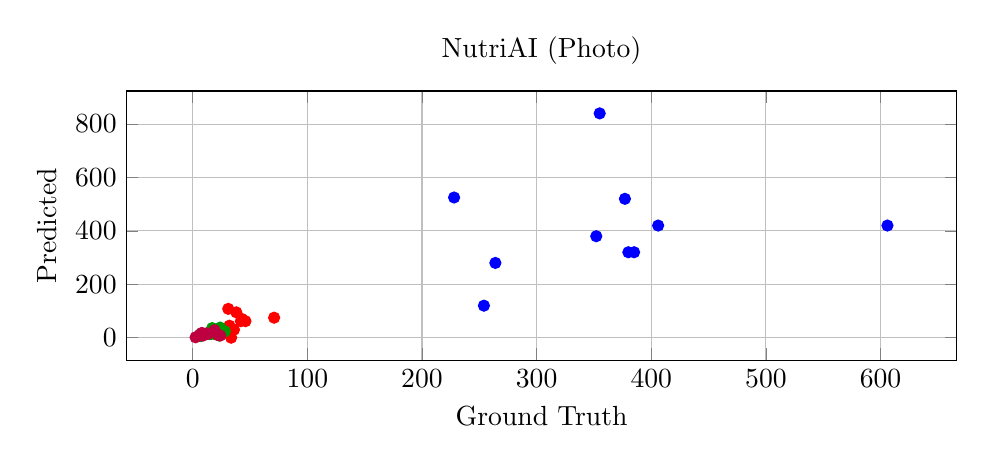
\begin{tikzpicture}
\begin{axis}[
    width=\linewidth,
    height=5cm,
    xlabel={Ground Truth},
    ylabel={Predicted},
    grid=major,
    title={NutriAI (Photo)}
]
% Calories
\addplot[only marks, blue] coordinates {
(377,520) (385,320) (406,420) (606,420) (228,525)
(264,280) (352,380) (254,120) (355,840) (380,320)
};
% Carbs
\addplot[only marks, red] coordinates {
(42,62) (31,26) (43,70) (71,75) (38,95)
(36,30) (46,62) (33.5,0) (31,108) (32,45)
};
% Protein
\addplot[only marks, green!60!black] coordinates {
(24,38) (16,14) (7,14) (19,14) (9,12)
(7,6) (23,8) (28,24) (17,36) (15,14)
};
% Fat
\addplot[only marks, purple] coordinates {
(13,14) (8,18) (9,8) (24,8) (6,10)
(12,16) (9,12) (2.5,1.5) (19,28) (22,10)
};
\end{axis}
\end{tikzpicture}
\caption{NutriAI — Photo}
\end{subfigure}
\hfill
\begin{subfigure}{0.48\textwidth}
\centering
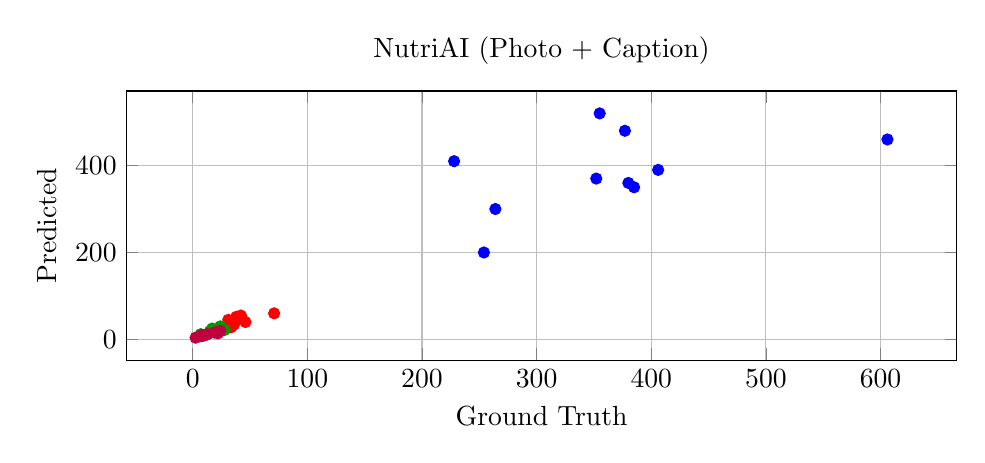
\begin{tikzpicture}
\begin{axis}[
    width=\linewidth,
    height=5cm,
    xlabel={Ground Truth},
    ylabel={Predicted},
    grid=major,
    title={NutriAI (Photo + Caption)}
]
\addplot[only marks, blue] coordinates {
(377,480) (385,350) (406,390) (606,460) (228,410)
(264,300) (352,370) (254,200) (355,520) (380,360)
};
\addplot[only marks, red] coordinates {
(42,55) (31,29) (43,48) (71,60) (38,52)
(36,34) (46,40) (33.5,28) (31,45) (32,37)
};
\addplot[only marks, green!60!black] coordinates {
(24,30) (16,18) (7,12) (19,16) (9,10)
(7,8) (23,18) (28,22) (17,25) (15,19)
};
\addplot[only marks, purple] coordinates {
(13,12) (8,10) (9,8) (24,20) (6,7)
(12,11) (9,10) (2.5,4) (19,16) (22,14)
};
\end{axis}
\end{tikzpicture}
\caption{NutriAI — Photo + Caption}
\end{subfigure}

\vspace{0.4cm}

% ---------- ROW 2: Other apps ----------
\begin{subfigure}{0.32\textwidth}
\centering
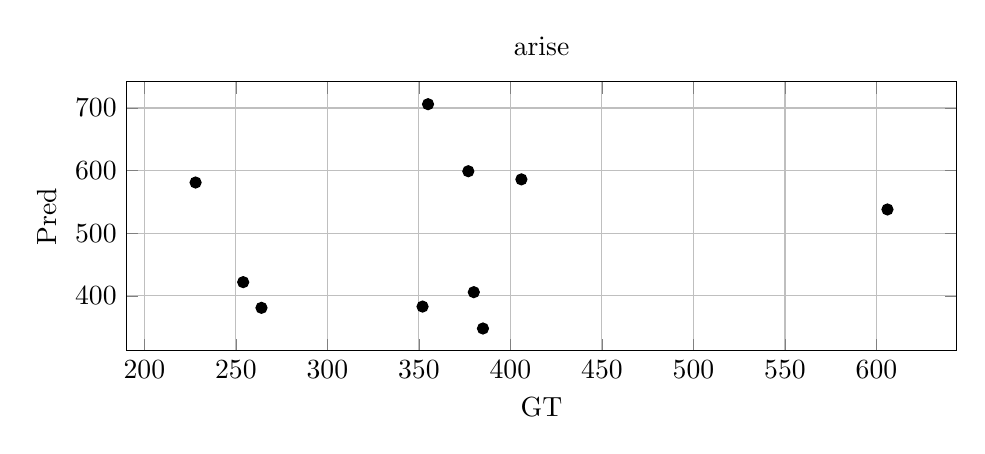
\begin{tikzpicture}
\begin{axis}[
    width=\linewidth,
    height=5cm,
    xlabel={GT},
    ylabel={Pred},
    grid=major,
    title={arise}
]
\addplot[only marks] coordinates {
(377,599) (385,348) (406,586) (606,538) (228,581)
(264,381) (352,383) (254,422) (355,706) (380,406)
};
\end{axis}
\end{tikzpicture}
\end{subfigure}
\hfill
\begin{subfigure}{0.32\textwidth}
\centering
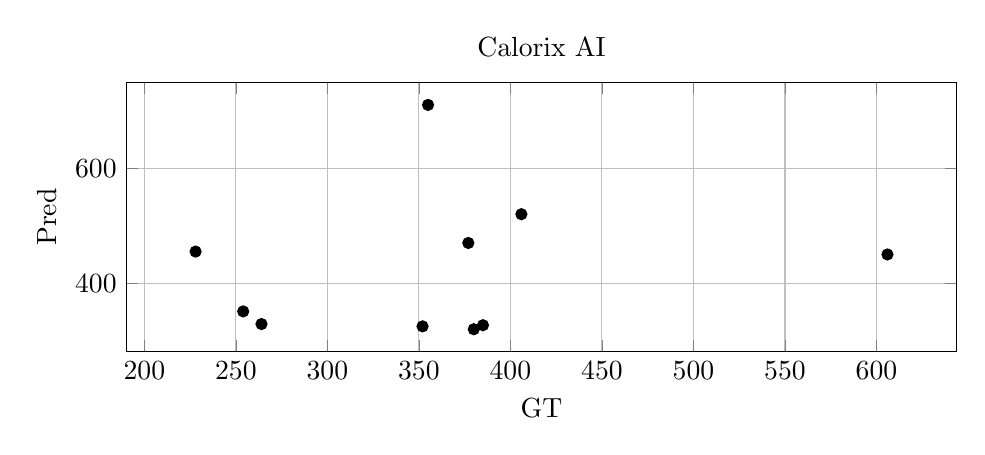
\begin{tikzpicture}
\begin{axis}[
    width=\linewidth,
    height=5cm,
    xlabel={GT},
    ylabel={Pred},
    grid=major,
    title={Calorix AI}
]
\addplot[only marks] coordinates {
(377,470) (385,327) (406,520) (606,450) (228,455)
(264,329) (352,325) (254,351) (355,710) (380,320)
};
\end{axis}
\end{tikzpicture}
\end{subfigure}
\hfill
\begin{subfigure}{0.32\textwidth}
\centering
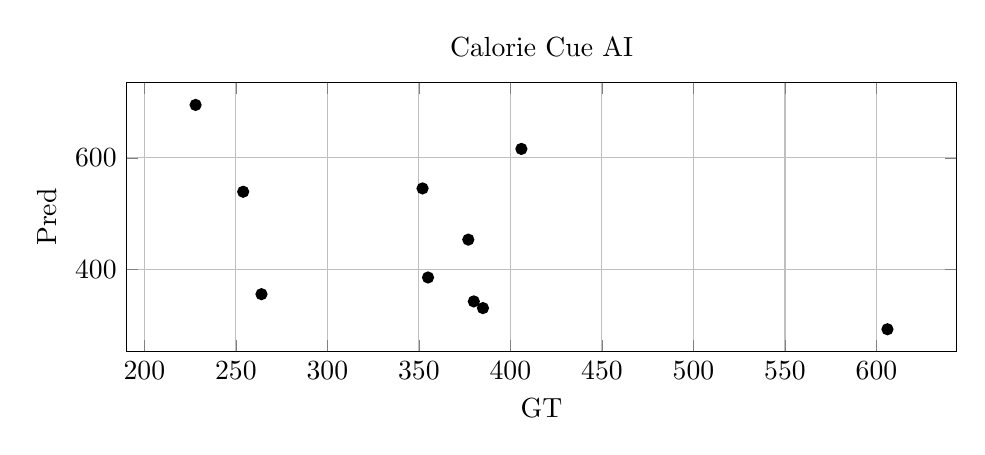
\begin{tikzpicture}
\begin{axis}[
    width=\linewidth,
    height=5cm,
    xlabel={GT},
    ylabel={Pred},
    grid=major,
    title={Calorie Cue AI}
]
\addplot[only marks] coordinates {
(377,453) (385,330) (406,616) (606,292) (228,695)
(264,355) (352,545) (254,539) (355,385) (380,342)
};
\end{axis}
\end{tikzpicture}
\end{subfigure}

\caption{Scatter plots comparing ground-truth and estimated nutritional values across applications (photo-only and photo+caption input).}
\label{fig:scatter_all_apps_extended}
\end{figure}

\begin{figure}[H]
\centering

% ---------- CALORIES ----------
\begin{subfigure}{0.48\textwidth}
\centering
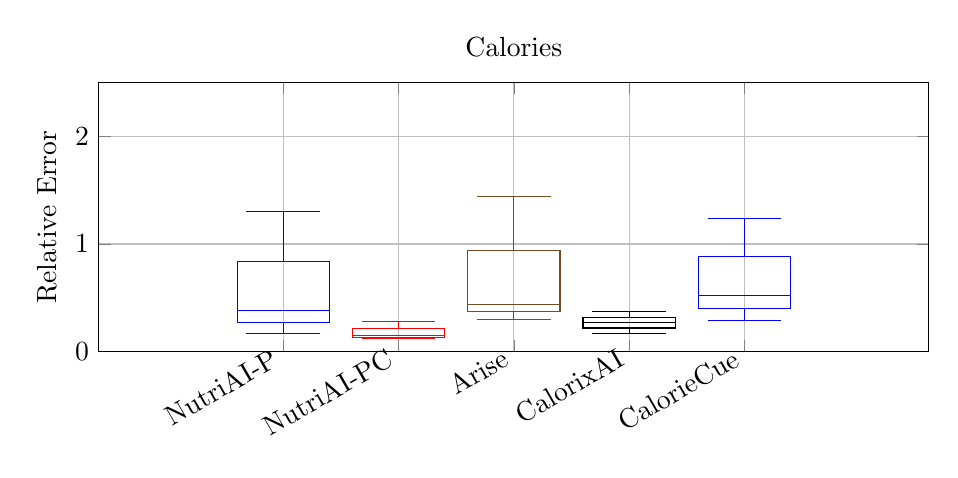
\begin{tikzpicture}
\begin{axis}[
  title={Calories},
  boxplot/draw direction=y,
  width=\textwidth,
  height=5cm,
  ymin=0, ymax=2.5,
  ylabel={Relative Error},
  xtick={1,2,3,4,5},
  xticklabels={NutriAI-P, NutriAI-PC, Arise, CalorixAI, CalorieCue},
  x tick label style={rotate=30, anchor=east},
  enlarge x limits=0.25,
  grid=major
]

\addplot+ [boxplot] coordinates {(0,0.38) (0,0.17) (0,1.30)};
\addplot+ [boxplot] coordinates {(1,0.15) (1,0.12) (1,0.28)};
\addplot+ [boxplot] coordinates {(2,0.44) (2,1.44) (2,0.30)};
\addplot+ [boxplot] coordinates {(3,0.27) (3,0.37) (3,0.17)};
\addplot+ [boxplot] coordinates {(4,0.52) (4,1.24) (4,0.29)};

\end{axis}
\end{tikzpicture}
\caption{Calories}
\end{subfigure}
\hfill

% ---------- CARBOHYDRATES ----------
\begin{subfigure}{0.48\textwidth}
\centering
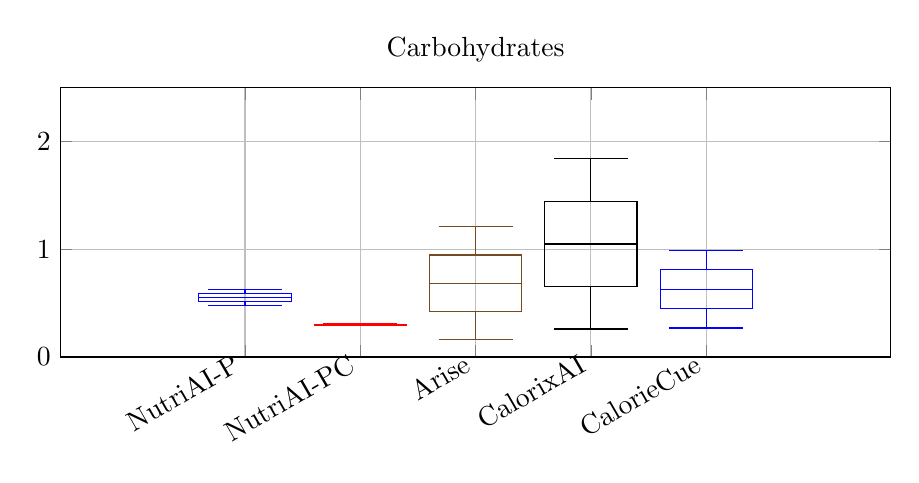
\begin{tikzpicture}
\begin{axis}[
  title={Carbohydrates},
  boxplot/draw direction=y,
  width=\textwidth,
  height=5cm,
  ymin=0, ymax=2.5,
  xtick={1,2,3,4,5},
  xticklabels={NutriAI-P, NutriAI-PC, Arise, CalorixAI, CalorieCue},
  x tick label style={rotate=30, anchor=east},
  enlarge x limits=0.25,
  grid=major
]

\addplot+ [boxplot] coordinates {(0,0.48) (0,0.63)};
\addplot+ [boxplot] coordinates {(1,0.31) (1,0.29)};
\addplot+ [boxplot] coordinates {(2,0.16) (2,1.21)};
\addplot+ [boxplot] coordinates {(3,0.26) (3,1.84)};
\addplot+ [boxplot] coordinates {(4,0.99) (4,0.27)};

\end{axis}
\end{tikzpicture}
\caption{Carbohydrates}
\end{subfigure}

\vspace{0.4cm}

% ---------- PROTEIN ----------
\begin{subfigure}{0.48\textwidth}
\centering
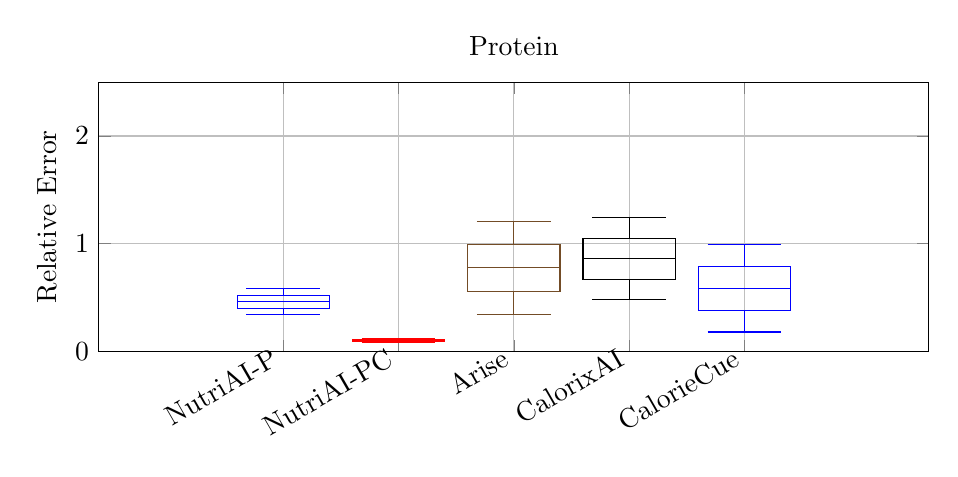
\begin{tikzpicture}
\begin{axis}[
  title={Protein},
  boxplot/draw direction=y,
  width=\textwidth,
  height=5cm,
  ymin=0, ymax=2.5,
  ylabel={Relative Error},
  xtick={1,2,3,4,5},
  xticklabels={NutriAI-P, NutriAI-PC, Arise, CalorixAI, CalorieCue},
  x tick label style={rotate=30, anchor=east},
  enlarge x limits=0.25,
  grid=major
]

\addplot+ [boxplot] coordinates {(0,0.58) (0,0.34)};
\addplot+ [boxplot] coordinates {(1,0.08) (1,0.12)};
\addplot+ [boxplot] coordinates {(2,0.34) (2,1.21)};
\addplot+ [boxplot] coordinates {(3,0.48) (3,1.24)};
\addplot+ [boxplot] coordinates {(4,0.18) (4,0.99)};

\end{axis}
\end{tikzpicture}
\caption{Protein}
\end{subfigure}
\hfill

% ---------- FAT ----------
\begin{subfigure}{0.48\textwidth}
\centering
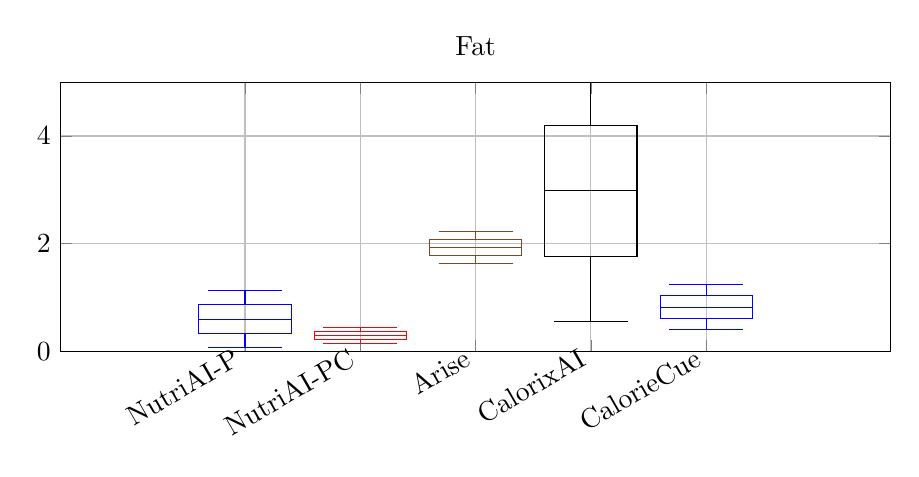
\begin{tikzpicture}
\begin{axis}[
  title={Fat},
  boxplot/draw direction=y,
  width=\textwidth,
  height=5cm,
  ymin=0, ymax=5,
  xtick={1,2,3,4,5},
  xticklabels={NutriAI-P, NutriAI-PC, Arise, CalorixAI, CalorieCue},
  x tick label style={rotate=30, anchor=east},
  enlarge x limits=0.25,
  grid=major
]

\addplot+ [boxplot] coordinates {(0,0.07) (0,1.13)};
\addplot+ [boxplot] coordinates {(1,0.14) (1,0.45)};
\addplot+ [boxplot] coordinates {(2,1.63) (2,2.22)};
\addplot+ [boxplot] coordinates {(3,0.56) (3,5.40)};
\addplot+ [boxplot] coordinates {(4,1.24) (4,0.40)};

\end{axis}
\end{tikzpicture}
\caption{Fat}
\end{subfigure}

\caption{Distribution of relative estimation error (MAPE) across applications and nutrients}
\label{fig:boxplots_all_nutrients}
\end{figure}

After analyzing the metrics: 

Nutri AI with photo input only demonstrates a reasonable linear tendency for calories and macronutrients, even though for meal with higher energetic values it demonstrated a systematic overestimation. It showed sensibility to the visual complexity of the meal. 
Nutri AI with photo and caption input had the best results, being among all of the apps the one with smaller errors and closer points to the ideal diagonal. The caption addition reduces extreme mistakes, specially with protein and fat. 
Arise app tends to overestimate calories and fat with high dispersion. 
Calorix AI shows a high variability and significant errors in energetic meals, specially in carbs, the dispersion suggests strong dependence in internal portion assumptions. 
Calorie Cue AI presents notable outlier with some estimations far from the GT. The performance quickly deteriorates with meal over 400kcal. 

Even with photo only NutriAI app outperformed the other apps. 

The box plots show that fro calories NutriAI (photo input only) presents the lower median, IQR and the less extreme outlier. On the other hand arise and CalorixAI present the higher medians and longer tails meaning higher errors. Carbs is the nutrient with the higher variability in general Nutri AI (photo input only) keeps the errors relatively controlled, while CalorieCue AI presents a big dispersion representative of a low accuracy in carbs. For proteins both versions of NutriAI (photo input only and photo + caption input) show a good stability, the other apps show asymmetric distributions suggesting difficulty in estimate protein sources with an image. Fat is the nutrients with higher relative erros in all of the apps. arise and CalorixAI present extreme outliers, while NutriAI (photo and caption input) has a significantly lower variability. 
The quantitative error analysis confirms the qualitative trends observed in the scatter and box plots. NutriAI with photo-only input achieves the lowest relative error for calories (34\%) and carbohydrates (49\%), while the photo + caption variant improves consistency across nutrients, particularly for protein (37\%) and fat (68\%). In contrast, Arise, Calorix AI, and Calorie Cue AI present substantially higher errors, especially for fat estimation, where relative deviations exceed 100\% in multiple cases. Overall, NutriAI demonstrates the most balanced and robust performance across macronutrients, and the inclusion of textual context proves beneficial in reducing estimation ambiguity and extreme deviations.




\section{Appendix- Table summary}
\subsection{General Summary}

\begin{table}[H]
\centering
\caption{High-level comparison of evaluated calorie and nutrient tracking applications}
\label{tab:apps_overview}
\begin{tabularx}{\textwidth}{Xccccc} % X faz a primeira coluna ocupar o espaço restante
\hline
\textbf{Feature} & \textbf{MFP} & \textbf{Arise} & \textbf{Calorix} & \textbf{C. Cue} & \textbf{NutriAI} \\
\hline
Verified food entries & Yes & Yes & No & Yes & No \\
User-generated foods & Yes & No & Yes & No & No \\
Photo-based meal scan & Paid & Free & Paid & Free & Yes \\
Barcode scanning & Free & Free & Limited & Limited & No \\
AI-assisted logging & Limited & Yes & Yes & Yes & Yes\\
Save AI-generated meals & Yes & No & Yes & No & Yes\\
Manual portion control & Yes & Limited & Limited & No & No\\
Free-tier usability & Med. & Med. & Low & Med. & NA\\
UX clarity & High & Med. & Low & Low & NA \\
Data export / API & Lim. & No & No & No & NA \\
\hline
\end{tabularx}
\end{table}

\section{Use of AI}
Generative AI tools were used as supporting assistants during this project to help with text structuring, language refinement, LaTeX formatting, and visualization setup. All benchmarking activities, experimental design, data collection, analysis, and interpretation of results were performed by the author, with GenAI outputs being critically reviewed and edited before inclusion. The use of GenAI was therefore complementary and did not replace analytical reasoning or decision-making.

\end{document}
